\chapter{Brevísima historia de la Ciencia}
\label{cha:historiaciencia}

\begin{enestecapitulo}
	\item[\emoji{classical-building}] Cómo entendían el mundo los primeros filósofos.
	\item[\emoji{telescope}] Cómo afectó a la ciencia la experimentación y la observación.
	\item[\emoji{atom-symbol}] Por qué la relatividad y la cuántica revolucionaron la física.
	\item[\emoji{robot}] Cómo la computación está transformando lo que significa hacer ciencia.
\end{enestecapitulo}

¿Cómo empezó todo esto que hoy llamamos “ciencia”?
¿Quiénes fueron los personajes que, con sus aciertos y sus errores, construyeron el edificio del conocimiento científico tal como lo conocemos?

Este capítulo es un recorrido rápido —una brevísima historia— por los hitos que marcaron el camino desde las primeras especulaciones de los filósofos griegos hasta la ciencia interdisciplinaria y computarizada del siglo~\textsc{xxi}.
No pretendemos ser exhaustivos (para eso existen libros enteros), sino trazar un mapa que te permita ubicar en el tiempo las ideas que discutiremos en los capítulos siguientes.

\begin{digress}{¿Por qué estudiar la historia de la ciencia?}
	Conocer la historia de la ciencia no es un mero ejercicio de erudición.
	Entender \emph{cómo} surgieron las teorías que hoy damos por sentadas nos ayuda a comprender \emph{por qué} las aceptamos, y nos vacuna contra la idea ingenua de que la ciencia es un camino recto y sin tropiezos hacia la verdad.
	La ciencia real está llena de callejones sin salida, de genios que se equivocaron y de accidentes afortunados.
\end{digress}

\section{La ciencia en la antigüedad}
\label{sec:cienciaenlaantiguedad}

Desde la antigua Grecia, los filósofos se preguntaban por las causas del mundo.
Tal es el caso de \person{Aristóteles} (384--322 a. C.), quien propuso muchas teorías físicas basándose en acertijos conceptuales y razonamientos lógicos, pero sin experimentación ni observación\cite{Shields2023}.
Su \index{física}\emph{física} se basaba en la idea de que la naturaleza busca siempre la economía y la perfección.

Por ejemplo, él afirmaba que los planetas giran en círculos porque este es el movimiento más perfecto, y que los objetos caen al suelo porque buscan su lugar natural, más aún, que los objetos más pesados caen más rápido.
A esta cosmovisión se le conoce como \emph{aristotelismo}, y fue la base del conocimiento científico hasta el siglo \textsc{xvii}.

\begin{remember}
	\label{rem:aristotelismo}
	El \terminology[aristotelismo]{aristotelismo} es la cosmovisión que enfatiza
	la importancia de la lógica y la razón para entender el mundo.
\end{remember}

Parte central del aristotelismo fue la \index{teoría!geocéntrica}teoría geocéntrica, introducida por \person{Ptolomeo} (90--168 d. C.).
Esta teoría postula que la Tierra es el centro del universo y que todos los demás cuerpos celestes giran alrededor de ella.

\begin{figure}[ht]
	\centering
	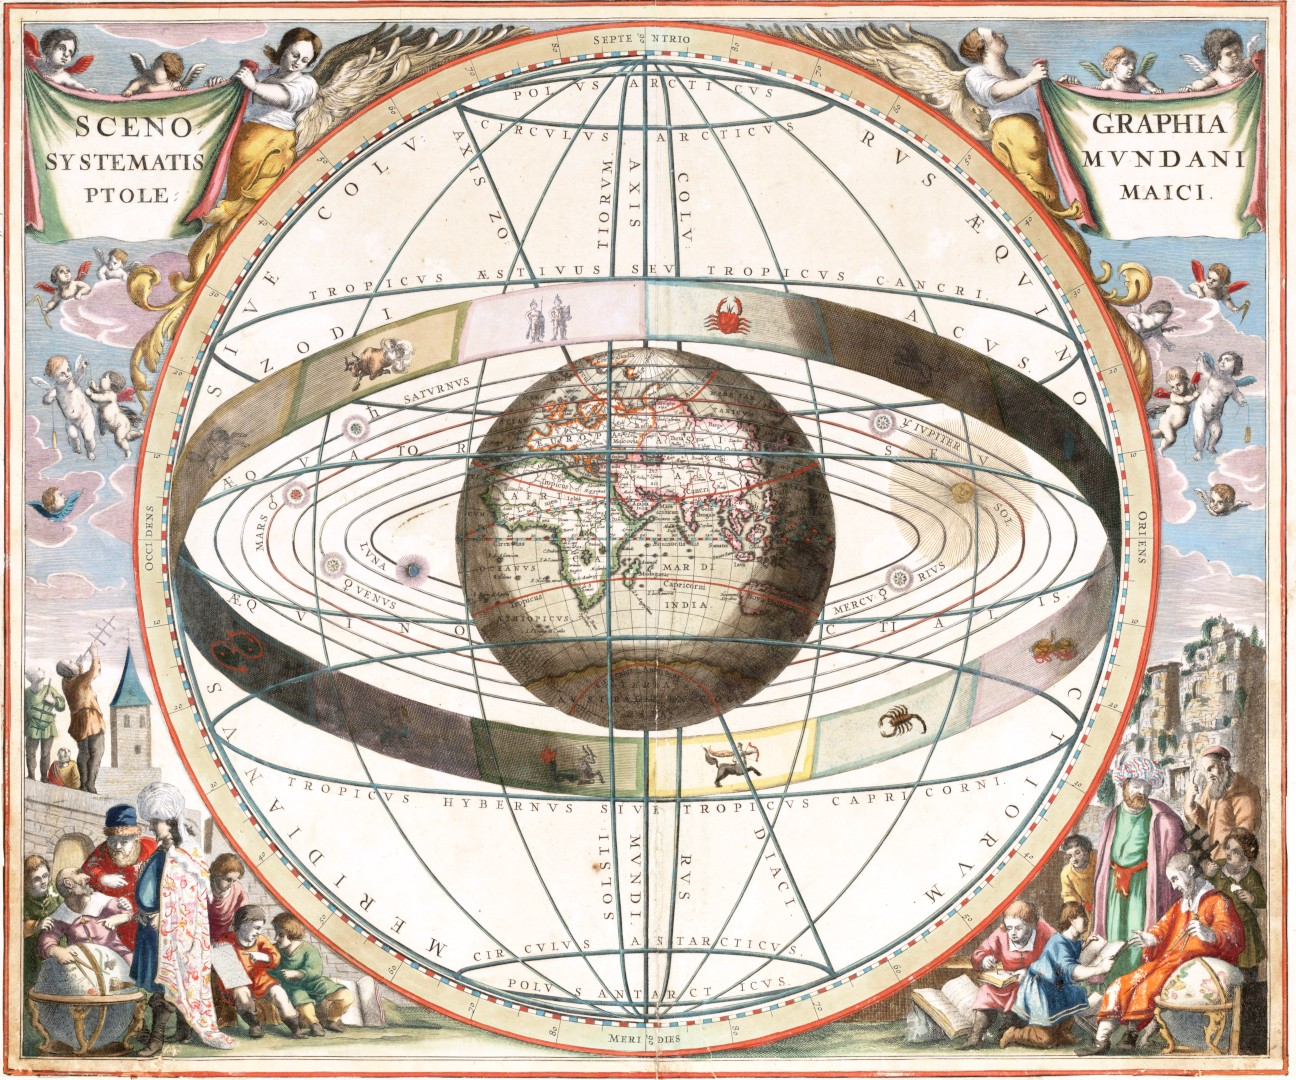
\includegraphics[width=0.8\linewidth]{img/Cellarius_ptolemaic_system}
	\caption{El sistema ptolemaico, en el que la Tierra es el centro del
		universo. Crédito: Loon, J. van (Johannes), aprox. 1611--1686 /
		Dominio público.}
	\label{fig:ptolemaico}
\end{figure}

\begin{digress}{¿Sabías que…?}
	Aunque hoy nos parezca ingenua, la física de Aristóteles \emph{funcionaba} para explicar el mundo cotidiano durante casi dos mil años.
	Si sueltas una piedra, cae; si empujas un carro, se detiene cuando dejas de empujarlo.
	El problema no era que Aristóteles estuviera completamente equivocado, sino que sus explicaciones eran \emph{aproximaciones} válidas solo en ciertas condiciones.
\end{digress}

\section{La revolución científica}
\label{sec:larevolucioncientifica}

Fue hasta 1542 cuando el canónigo católico \person[Copérnico]{Nicolás} (1473--1543) se atrevió a desafiar el aristotelismo publicando su libro \emph{De revolutionibus orbium coelestium} (Sobre las revoluciones de las esferas celestes), en el que propone que el Sol está fijo en el centro del universo y que los planetas giran alrededor de él, dando lugar así a la \index{teoría!heliocéntrica}\emph{teoría heliocéntrica}.

La teoría no fue bien recibida por la Iglesia, ni aún cuando su autor la dedicó al Papa Pablo \textsc{iii}.
Más bien fue vetada de 1616 a 1835, pero en solo cien años se había convertido en la teoría dominante gracias a los trabajos de \person{Galileo Galilei} (1564--1642) y \person{Johannes Kepler} (1571--1630).
Kepler descubrió que los planetas se mueven en órbitas elípticas y no circulares como creía Copérnico, y así resolvió el problema de la posición de Marte en el cielo nocturno.
En cambio, Galileo apuntó su telescopio al cielo y descubrió que Júpiter tiene cuatro lunas, que la Luna tiene montañas y cráteres, y que el Sol tiene manchas entre otras cosas.

Galileo también hizo importantes contribuciones en otras áreas de la ciencia; descubrió la \emph{ley de caída de los cuerpos}, que dice que todos los cuerpos caen con la misma aceleración.
Según relata su discípulo Vivianni, esto lo demostró dejando caer dos bolas de diferente peso desde lo alto de la Torre inclinada de Pisa \cite{Viviani2019}.
Hasta entonces la lógica aristotélica era suficiente para explicar el mundo, la experimentación era considerada una actividad de segunda clase, y las matemáticas servían para describir objetos ideales pero no la realidad.
Galileo cambió todo esto, y por ello se le considera el primer científico moderno.
Desafortunadamente, Galileo fue condenado por la Inquisición en 1633 por defender a la teoría heliocéntrica, que para entonces era considerada herética por contradecir la creación del mundo descrita en la Biblia.
Él pasó el resto de su vida bajo arresto domiciliario y se convirtió así también en el ejemplo más famoso del conflicto entre ciencia y religión.

Luego de la muerte de Galileo, la ciencia entró en una etapa de rápido avance.
\person[Descartes]{René} (1596--1650), con su \emph{mecanicismo}, propuso que el universo es como una maquinaria de reloj en la que todo puede explicarse en términos del movimiento y colisión de partículas.
Asimismo, en su \emph{Discurso del método} (1637) propuso que la ciencia debe basarse en la razón y no en la autoridad, y que la experimentación y la observación son las herramientas más importantes para el científico.

\begin{remember}
	\label{rem:mecanicismo}
	El \terminology[mecanicismo]{mecanicismo} es la cosmovisión según la cual
	el universo se comporta como una maquinaria determinista, y que puede ser
	explicada en términos del movimiento y colisión de partículas.
\end{remember}

Por su parte, \person[Newton]{Isaac} (1643--1727) propuso sus tres leyes del movimiento y la ley de la gravitación universal, que explica la atracción entre los cuerpos celestes.
Su obra maestra intitulada \emph{Philosophiae Naturalis Principia Mathematica} (Principios matemáticos de la filosofía natural) se publicó en 1687, y fue el marco teórico de referencia para la ciencia durante los siguientes 200 años.
Esta teoría sería extendida por muchos otros científicos para explicar más fenómenos, como la mecánica de fluidos o la teoría electromagnética.

\begin{figure}[ht]
	\centering
	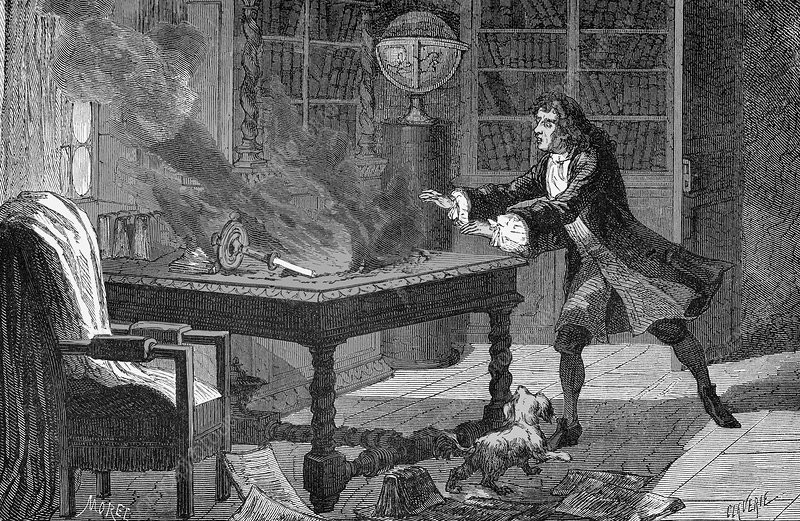
\includegraphics[width=0.8\linewidth]{img/Isaac_Newton_laboratory_fire}
	\caption{Isaac Newton en su laboratorio.
		Su mascota \emph{Diamond} tiró una vela sobre una mesa de papeles,
		quemando varios años de trabajo en el proceso.
		Crédito: Morel / Dominio público.
	}

\end{figure}

Durante un par de siglos se consideró que la teoría de Newton era esencialmente correcta, y que los científicos sólo necesitaban rellenar meros detalles técnicos para completar el cuadro.

\begin{digress}{El relojero ciego}
	La imagen del universo como un reloj —una maquinaria perfecta puesta en marcha por un Creador y que funciona siguiendo leyes precisas— fue la metáfora dominante durante la Ilustración.
	Esta idea, conocida como \emph{deísmo}, reconciliaba la ciencia con la religión: Dios creó el universo con leyes perfectas, y la tarea del científico es descubrir esas leyes.
	Irónicamente, fue el éxito mismo de la física newtoniana lo que eventualmente hizo que muchos pensadores prescindieran de la hipótesis de Dios.
\end{digress}

\section{La ciencia moderna}
\label{sec:lacienciamoderna}

En 1859, \person[Darwin]{Charles} (1809--1882) publicó su libro \emph{El origen de las especies}, en el que propone la teoría de la evolución mediante la selección natural.
Ya se sabía que las especies cambian con el tiempo si se seleccionan artificialmente a los individuos más aptos para la reproducción en la agricultura y la ganadería, donde se habían obtenido nuevas variedades de plantas y animales más aptas para el consumo humano.
Darwin propuso que este mismo proceso ocurre en la naturaleza, donde las especies co-evolucionan con su entorno y se adaptan a él.

A mediados del siglo \textsc{xix} el físico escocés \person[Maxwell]{James} (1831--1879) descubrió que la luz es una onda electromagnética que se propaga a la velocidad de la luz, unificando así las teorías de la electricidad y el magnetismo.
Esto fue un gran avance, pero también un problema, pues las ecuaciones de Maxwell entran en conflicto con la mecánica Newtoniana cuando se consideran altas velocidades.
El final del siglo \textsc{xix} y el principio del \textsc{xx} fueron testigos de invenciones increíbles como el teléfono, la radio, y el avión, pero también de descubrimientos científicos que cimbraron la visión mecanicista del mundo.
En 1905, \person[Einstein]{Albert} (1879--1955) publicó su \emph{teoría de la relatividad especial}, en la que propuso que el tiempo y el espacio son relativos, y que la velocidad de la luz es la misma para todos los observadores.

Por otro lado, apareció el problema de la \emph{radiación del cuerpo opaco}, que desafiaba la física clásica al intentar comprender cómo un objeto caliente emite radiación electromagnética.
Las predicciones clásicas indicaban que bajo ciertas condiciones este emitiría radiación infinita, en clara contradicción con las observaciones experimentales.
Este problema fue resuelto por \person[Planck]{Max} (1858--1947) en 1900, quien propuso que la energía se emite en paquetes discretos llamados \emph{cuantos}, dando origen a la \index{mecánica cuántica}mecánica cuántica.

En conjunto, la teoría de la relatividad y la mecánica cuántica revolucionaron la física y la ciencia en general, disminuyendo la confianza en la teoría de Newton y en el método científico clásico.
Ambas teorías son tan extrañas como exitosas, y han sido confirmadas por miles de experimentos, pero aún así son difíciles de entender y de aceptar.

Para este entonces, la ciencia ya se hacía de forma colaborativa, las cartas se publicaban en revistas científicas, y los científicos se reunían en conferencias para discutir sus ideas.
Uno de estos grupos, el \index{círculo de Viena}\emph{círculo de Viena}, se reunió a discutir la naturaleza de la ciencia, y en 1929 publicaron su \emph{Manifiesto científico}, donde expresa la visión científica del mundo que se basa en el empirismo, la lógica y el análisis del lenguaje.
El manifiesto propone que la filosofía se ocupe de clarificar los conceptos y los criterios de la ciencia, y que rechace la metafísica como una pseudociencia sin sentido.

\begin{remember}
	\label{rem:empirismo lógico}
	El \terminology[empirismo!lógico]{empirismo lógico} es una corriente
	filosófica que sostiene que el único conocimiento válido es el que se basa
	en la experiencia, la observación y la lógica.
	Una afirmación que no tiene contenido empírico o lógico es considerada
	\emph{metafísica}, y por lo tanto no tiene sentido.
\end{remember}

En 1936, \person[Turing]{Alan} (1912--1954) publicó su artículo \emph{On computable numbers, with an application to the Entscheidungsproblem}, en el que propuso una teoría acerca de las limitaciones de lo que se puede calcular...
En el proceso sentó las bases de la \index{computación}computación como disciplina científica.
Aquí se estudia el alcance y los límites del tratamiento de la información de forma automática.
Pasarían varios años antes de que apareciera la primera computadora electrónica de propósito general \emph{ENIAC} (Electronic Numerical Integrator and Computer) en 1946.
\begin{figure}[ht]
	\centering
	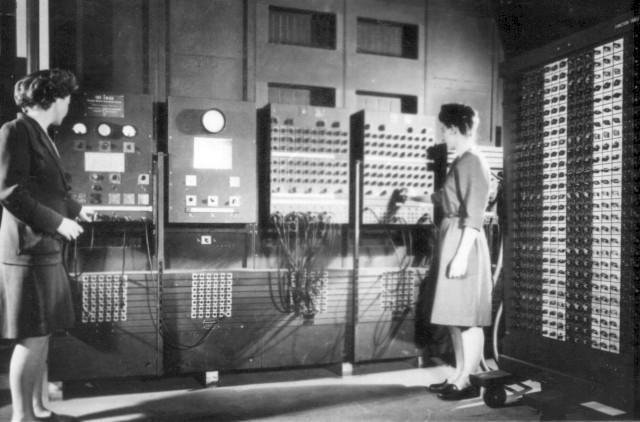
\includegraphics[width=0.8\linewidth]{img/Two_women_operating_ENIAC}
	\caption{Dos mujeres operando la computadora ENIAC.
		Aunque a menudo se omite en los libros de texto, muchas de las primeras programadoras fueron mujeres, un hecho que la historia de la computación está apenas comenzando a reconocer.
		Crédito: U.S. Army Photo / Dominio público.
	}
\end{figure}

Para 1953, \person[Watson]{James} (1928--) y \person[Crick]{Francis} (1916--2004) descubrieron la estructura del ácido desoxirribonucleico (ADN), la molécula que contiene la información genética de los seres vivos, dando inicio a la \index{biología!molecular}biología molecular que estudia los procesos biológicos en términos de las moléculas que los componen.
Esta disciplina se ha desarrollado rápidamente gracias a la computación, que permite simular y analizar los procesos biológicos a nivel molecular.
En 2003 se completó el \index{Proyecto Genoma Humano}Proyecto Genoma Humano, que consistió en secuenciar el ADN de un ser humano, y que ha permitido entender mejor las enfermedades genéticas y desarrollar nuevos tratamientos médicos.

\begin{figure}[ht]
	\centering
	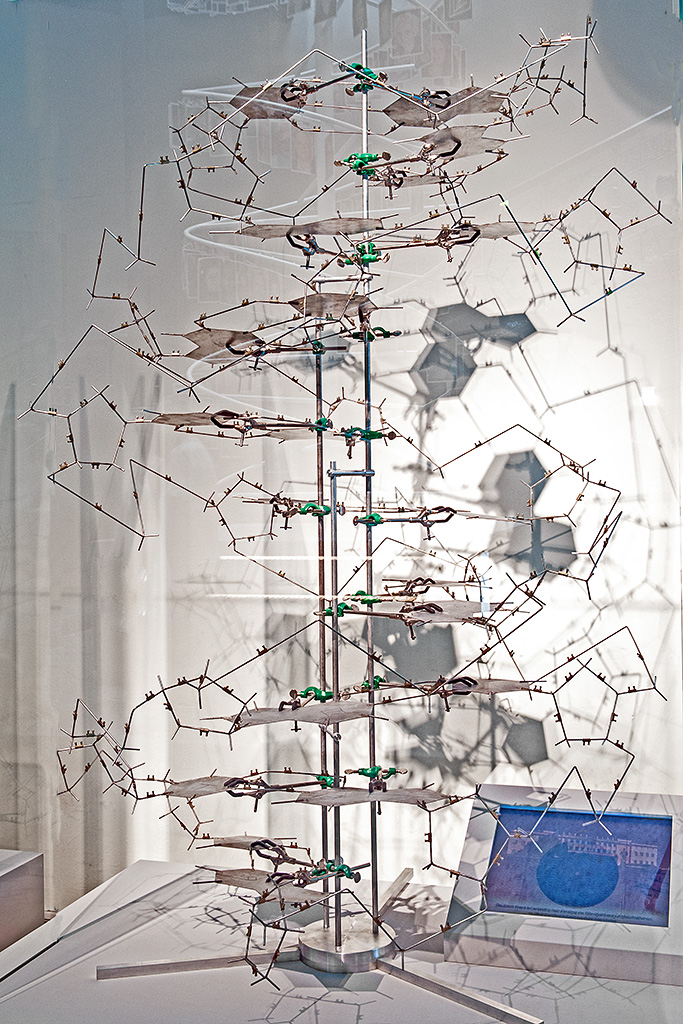
\includegraphics[height=0.618\textheight]{img/60_Jahre_DNA_01.jpg}
	\caption{Réplica del modelo de ADN de Watson y Crick.
		Crédito: Museum für Naturkunde Berlin.}
	\label{fig:dna}
\end{figure}

\section{La ciencia contemporánea}
\label{sec:lacienciacontemporanea}

El siglo \textsc{xx} fue testigo de la creación o formalización de disciplinas como \index{economía}economía, \index{antropología}antropología, \index{sociología}sociología, \index{psicología}psicología, y \index{lingüística}lingüística.
En general, estas disciplinas se basan en el método científico, pero no son ciencias naturales.
Por ejemplo, la sociología estudia la sociedad y la cultura, pero es mayormente una ciencia observacional, pues no se pueden hacer experimentos con sociedades humanas.

La tendencia actual es la \emph{interdisciplinariedad}, es decir, la colaboración entre diferentes disciplinas.
Esto fue facilitado por la computación, que es usada como herramienta en todas partes.
Por ejemplo, la climatología estudia el clima de la Tierra, y para ello simula el comportamiento de la atmósfera mediante modelos computacionales.
Sin embargo, estos métodos de simulación cuestionan la naturaleza misma de la ciencia: ¿Es válido un conocimiento científico que no se basa en la experimentación ni en la observación, pero que es capaz de predecir el comportamiento de un fenómeno observado?

\begin{remember}
	\label{rem:interdisciplinariedad}
	La \terminology{interdisciplinariedad} es la colaboración entre diferentes
	disciplinas para resolver un problema, y es la base de la ciencia moderna.
\end{remember}

En este período también se desarrolló la inteligencia artificial, que estudia la creación de máquinas inteligentes.
En 1977 los matemáticos Kenneth Appel y Wolfgang Haken usaron una computadora para demostrar el \emph{teorema de los cuatro colores}, que dice que cualquier mapa puede ser coloreado con solo cuatro colores de forma que dos países vecinos no tengan el mismo color.
En su momento, esta demostración fue muy polémica, pues no se consideraba que una demostración computacional fuera válida.
Actualmente programas de computadora juegan ajedrez, conducen automóviles, diagnostican enfermedades, descubren exoplanetas, predicen la estructura de proteínas, y descubren nuevos materiales.
Algunos científicos cuestionan si estas actividades se pueden considerar inteligentes, ya que las máquinas no entienden lo que hacen, sino que siguen instrucciones programadas por humanos.
Entonces ¿son estos descubrimientos computarizados \emph{científicos}?
¿La naturaleza del conocimiento científico ha cambiado con la computación?

\begin{remember}
	\label{rem:historia-preguntas}
	A lo largo de este brevísimo recorrido hemos visto que la ciencia no siempre fue como la conocemos hoy.
	Pasó de ser una actividad especulativa en la antigüedad, a una empresa experimental en la revolución científica, a una disciplina colaborativa e interdisciplinaria en la actualidad.
\end{remember}

En el siguiente capítulo nos preguntaremos: ¿qué es, exactamente, eso que llamamos “ciencia”?
¿Hay algo que todas estas épocas y disciplinas tengan en común?
¿O será que la ciencia es simplemente lo que los científicos hacen?
Volveremos a estas preguntas cuando exploremos el problema de demarcación y el falsacionismo de Popper, que intentan trazar justamente esa frontera entre lo que es ciencia y lo que no.
